\chapter{Probabilistic Planning with Sequential Monte Carlo Methods}
\section{Appendix}
\label{sec:appendix}

\subsection{Abbreviation and Notation}
\label{app:notation}
\begin{table}[H]\caption{Abbreviation}
\begin{center}% used the environment to augment the vertical space
% between the caption and the table
\begin{tabular}{r c p{10cm} }
\toprule
SMCP: & Sequential Monte Carlo Planning.\\
SAC: & Soft Actor Critic.\\
CEM: & Cross Entropy Method.\\
RS: & Random Shooting.\\
MCTS: & Monte Carlo Tree Search.\\
SMC: & Sequential Monte Carlo.\\
SIR: & Sequential Importance Resampling.\\
SIS: & Sequential Importance Sampling.\\
IS: & Importance Sampling.\\
MPC: & Model Predictive Control\\
\bottomrule
\end{tabular}
\end{center}
\label{tab:abbreviation}
\end{table}

\begin{table}[H]\caption{Notation}
\begin{center}% used the environment to augment the vertical space
% between the caption and the table
\begin{tabular}{r c p{10cm} }
\toprule
$\traj_{1:T}$ & $\triangleq$ & $\{\rvs_i, \rva_i\}_{i=1}^T$ the state-action pairs.\\
$V$  & $\triangleq$ & value function.\\
$\mathcal{O}_t$ & $\triangleq$ & Optimality variable.\\
$p(\mathcal{O}_t|\rvs_t, \rva_t)$ & $\triangleq$ & $\exp(r(\rvs_t, \rva_t))$ Probability of a pair state action of being optimal.\\
$\penv$ & $\triangleq$ & Transition probability of the environment. Takes state and action $(\rvs_t, \rva_t)$ as argument and return next state and reward $(\rvs_{t+1}, r_t)$.\\
$\pmodel$ & $\triangleq$ & Model of the environment. Takes state and action $(\rvs_t, \rva_t)$ as argument and return next state and reward $(\rvs_{t+1}, r_t)$.\\
% $w$ & $\triangleq$ & Unnormalized weight of the importance sampling.\\ 
% $\bar{w}$ & $\triangleq$ & Normalized weight of the importance sampling.\\
$w_t$ & $\triangleq$ & Importance sampling weight.\\ 
% $w_{t|T}$ & $\triangleq$ & Smoothing importance sampling weight.\\ 
$p(\traj)$  & $\triangleq$ & Density of interest.\\
$q(\traj)$  & $\triangleq$ & Approximation of the density of interest.\\
$t \in \{1, \ldots T\}$ & $\triangleq$ & time steps. \\
$n \in \{1, \ldots N\}$ & $\triangleq$ & particle number. \\
$h$ & $\triangleq$ & horizon length. \\
\bottomrule
\end{tabular}
\end{center}
\label{tab:notation}
\end{table}

%\subsection{Ablation Study}
%
%\begin{figure}
%    \centering
%    \includegraphics[angle=90,origin=c,scale=0.5]{ablation_study_halfcheetah}
%    \caption{Ablation study on half cheetah.}
%    \label{fig:my_label}
%\end{figure}

\subsection{The action prior}
\label{app:action_prior}

The true joint distribution~\ref{eq:posterior_target} in section~\ref{sec:control_as_inference} should actually be written:
\begin{eqnarray*}
\label{eq:true_posterior_target}
p(\traj_{1:T}, \gO_{1:T}) &=& \mu(\rvs_1) \prod_{t=1}^{T-1} \penv(\rvs_{t+1}|\rva_t, \rvs_t) \prod_{t=1}^{T} p(\rva_t) \exp\big(\sum_{t=1}^{T} r(\rvs_t, \rva_t)\big) \\
&=& \mu(\rvs_1) \prod_{t=1}^{T-1} \penv(\rvs_{t+1}|\rva_t, \rvs_t)\exp\big(\sum_{t=1}^{T} r(\rvs_t, \rva_t) + \log p(\rva_t)\big) \\
\end{eqnarray*}
In Mujoco environments, the reward is typically written as 
$$r(\rvs_t, \rva_t) = f(\rvs_t) - \alpha ||\rva_t||_2^2 $$
where $f$ is a function of the state (velocity for HalfCheetah on Mujoco for example). The part $\alpha ||\rva_t||_2^2$ can be seen as the contribution from the action prior (here a gaussian prior).
One can also consider the prior to be constant (and potentially improper) so that is does not change the posterior $p(\traj_{1:T}| \gO_{1:T})$.

% \subsection{Recursive filtering weights}

% \label{app:rec_weights}
% \begin{align}
% w_t &= \frac{p(\traj_{1:t} | \gO_{1:t})}{q(\traj_{1:t})} \nonumber\\
% &= \frac{p(\traj_{1:t-1} | \gO_{1:t-1}) \penv(\rvs_{t+1} | \rvs_t, \rva_t) p(\gO_t | \rvs_t, \rva_t)}{q(\traj_{1:t-1}) q(\traj_t | \traj_{1:t-1})} \nonumber\\
% &= \frac{p(\traj_{1:t-1} | \gO_{1:t-1}) }{q(\traj_{1:t-1}) }\frac{\penv(\rvs_{t+1} | \rvs_t, \rva_t) \exp(r_t)}{\pmodel(\rvs_{t+1} | \rvs_t, \rva_t) \pi_\parampol(\rva_t | \rvs_t)} \nonumber\\
% &= w_{t-1}\frac{\penv(\rvs_{t+1} | \rvs_t, \rva_t)}{\pmodel(\rvs_{t+1} | \rvs_t, \rva_t) } \exp(r_t - \log \pi_\parampol(\rva_t | \rvs_t))
% \end{align}

\subsection{Value function: backward message}
 \label{app:backward_message}
\begin{align}
    p(\gO_{t+1:T} | \traj_t) &=  \int_{\traj_{t+1}} p(\gO_{t+1:T}, \traj_{t+1} | \traj_t)d\traj_{t+1} \nonumber\\
     &=  \int_{\traj_{t+1}} p(\traj_{t+1} | \traj_{t}, \gO_{t+1:T}) p(\gO_{t+1:T} | \traj_{t+1}) d\traj_{t+1}  \nonumber\\
    % &= \int_{\traj_{t+1}} p(\traj_{t+1}|\traj_t) \exp Q(\rvs_{t+1}, \rva_{t+1}) d\traj_{t+1} \nonumber\\
     &= \int_{\rvs_{t+1}}  \penv(\rvs_{t+1} | \rvs_t, \rva_t) \left[ \int_{\rva_{t+1}} p(\rva_{t+1} | \rvs_{t+1}, \gO_{t+1:T}) \exp Q(\rvs_{t+1}, \rva_{t+1}) d\rva_{t+1}  \right] d\rvs_{t+1}\nonumber\\
     &= \int_{\rvs_{t+1}} \penv(\rvs_{t+1} | \rvs_t, \rva_t)  \exp \big( V(\rvs_{t+1}) \big) d\rvs_{t+1}\nonumber\\
       &= \E_{\rvs_{t+1} | \rvs_t, \rva_t} [ \exp \big( V(\rvs_{t+1}) \big)]
\end{align}
By definition of the optimal value function in~\citep{levine2018reinforcement}.


\subsection{Recursive weights update}
% {\color{red} Version with Q function}
% For this derivation, we need the forward backward equation
% \begin{align}
%     {p(\traj_{1:t} | \gO_{1:T})} & \propto \mathunderline{alpha}{p(\traj_{1:t}|\gO_{1:t})} \cdot \mathunderline{beta}{p(\gO_{t+1:T}|\traj_{t})}
% \end{align}
% and its alternative form
% \begin{align}
%     {p(\traj_{1:t} | \gO_{1:T})} & \propto \mathunderline{alpha}{p(\traj_{1:t}|\gO_{1:t-1})} \cdot \mathunderline{beta}{p(\gO_{t:T}|\traj_{t})}
% \end{align}


\label{app:rec_weights}
\begin{align}
w_t &= \frac{p(\traj_{1:t} | \gO_{1:T})}{q(\traj_{1:t})} \nonumber\\
&= \frac{p(\traj_{1:t-1} | \gO_{1:T})}{q(\traj_{1:t-1})}\frac{p(\traj_t |\traj_{1:t-1}, \gO_{1:T})}{q(\traj_t | \traj_{1:t-1})} \nonumber\\
&= w_{t-1} \cdot \frac{p(\traj_t |\traj_{1:t-1}, \gO_{1:T})}{q(\traj_t | \traj_{1:t-1})} \nonumber\\
&= w_{t-1} \frac{1}{ q(\traj_t | \traj_{1:t-1})} \frac{p(\traj_{1:t} | \gO_{1:T})}{ p(\traj_{1:t-1} | \gO_{1:T})} \nonumber\\
&\text{We use there the forward-backward equation~\ref{eq:forwardbackward} for the numerator and the denominator} \nonumber\\
 &\propto w_{t-1}   \frac{1}{ q(\traj_t | \traj_{1:t-1})} \frac{ \textcolor{orange}{p(\traj_{1:t} | \gO_{1:t})}}{ \textcolor{orange}{p(\traj_{1:t-1} | \gO_{1:t-1})}} \frac{ \textcolor{beta}{p(\gO_{t+1:T} | \traj_{t})}}{ \textcolor{beta}{p(\gO_{t:T} | \traj_{t-1})}}   \nonumber\\
&= w_{t-1}   \frac{ p(\traj_t | \traj_{1:t-1})}{ q(\traj_t | \traj_{1:t-1})}  p(\gO_t | \traj_t)   \frac{ p(\gO_{t+1:T} | \traj_{t})}{ p(\gO_{t:T} | \traj_{t-1})}  \nonumber\\
&= w_{t-1}    \frac{\penv(\rvs_{t} | \rvs_{t-1}, \rva_{t-1})}{ \pmodel(\rvs_{t} | \rvs_{t-1}, \rva_{t-1}) }   \frac{\exp (r_t)}{\pi_\parampol(\rva_t|\rvs_t)} \frac{\E_{\rvs_{t+1} | \rvs_t, \rva_t} [ \exp \big( V(\rvs_{t+1}) \big)] }{\E_{\rvs_{t} | \rvs_{t-1}, \rva_{t-1}} [ \exp \big( V(\rvs_{t}) \big)]}  \nonumber\\
% &= \frac{p(\traj_{1:t-1} | \gO_{1:t-1}) }{q(\traj_{1:t-1}) }\frac{\penv(\rvs_{t+1} | \rvs_t, \rva_t) \exp(r_t)}{\pmodel(\rvs_{t+1} | \rvs_t, \rva_t) \pi_\parampol(\rva_t | \rvs_t)} \nonumber\\
% &= w_{t-1}\frac{\penv(\rvs_{t+1} | \rvs_t, \rva_t)}{\pmodel(\rvs_{t+1} | \rvs_t, \rva_t) } \exp(r_t - \log \pi_\parampol(\rva_t | \rvs_t))
&= w_{t-1} \frac{\penv(\rvs_{t} | \rvs_{t-1}, \rva_{t-1})}{ \pmodel(\rvs_{t} | \rvs_{t-1}, \rva_{t-1}) }  \E_{\rvs_{t+1} | \rvs_t, \rva_t} [ \exp \big( r_t  -  \log \pi_\parampol(\rva_t | \rvs_t) + V(\rvs_{t+1}) - \log \E_{\rvs_{t} | \rvs_{t-1}, \rva_{t-1}} [ \exp \big( V(\rvs_{t}) \big)] \big)]
\end{align}


% As 
% $$p(\traj_{1:t} | \gO_{1:t}) = \mu(\rvs_1) \prod_{\tau=1}^{t-1} \penv(\rvs_{\tau+1}|\rva_\tau, \rvs_\tau) \exp\big(\sum_{\tau=1}^{t} r(\rvs_\tau, \rva_\tau) + \log p(\rva_\tau) \big)$$
% We have
% $$\frac{p(\traj_{1:t} | \gO_{1:t})}{ p(\traj_{1:t-1} | \gO_{1:t-1})}  = \penv(\rvs_{t} | \rvs_{t-1}, \rva_{t-1}) \exp\big( r(\rvs_t, \rva_t) + \log p(\rva_t) \big)$$

% Therefore we obtain
% \subsection{Residual Sampling}
% \label{app:res_sampling}

\subsection{Experiment Details}
\label{app:exp_details}

\paragraph{Random samples:} 1000 transitions are initially collected by a random policy to pretrain the model and the proposal distribution. After which the agents start following their respective policy.

\paragraph{Data preprocessing:} We normalize the observations to have zero mean and standard deviation 1. 

\paragraph{Model Predictive Control:} The model is used to predict the planning distribution for the horizon $h$ of $N$ particles. We then sample a trajectory according to its weight and return the first action of this trajectory. In our experiments, we fix the maximum number of particles for every method to 2500. For SMCP, the temperature and horizon length are described in Table~\ref{tbl:exp_hp}.

\paragraph{Soft Actor Critic:} We used a custom implementation with a Gaussian policy for both the SAC baseline and the proposal distribution used for both versions of SMCP. We used Adam \citep{kingma2014adam} with a learning rate of 0.001. The reward scaling suggested by \citet{haarnoja2018soft} for all experiments and used an implementation inspired by \citet{pong2018}. We used a two hidden layers with 256 hidden units for the three networks: the value function, the policy and the soft Q functions.

\paragraph{Model:} We train the model $\pmodel$ to minimize the negative log likelihood of $p(s_{t+1}|s_t + \Delta_t(s_t, a_t), \sigma_t(s_t, a_t))$. The exact architectures are detailed in Table~\ref{tbl:exp_hp}. We train the model to predict the distribution of the change in states and learn a deterministic reward function from the current state and predict the change in state. Additionally, we manually add a penalty on the action magnitude in the reward function to simplify the learning. At the end of each episode we train the model for 10 epochs. Since the training is fairly short, we stored every transitions into the buffer. The model is defined as:

\begin{align}
    \Delta s_{t} &\sim p(\cdot|s_t, a_t) \label{app:next_state}\\
    r_t &= g(s_t, \Delta s_t) - \alpha \|a\|^2 \label{app:reward_fct}
\end{align}


where $\alpha$ was taken from the Mujoco gym environments. We used Adam \citep{kingma2014adam} with a learning rate of 0.001 and leaky ReLU activation function.


\begin{table}[H]
\centering
\begin{tabular}{lcccc}
\toprule
\makecell{\bfseries Environment} & \thead{Temperature} & \thead{Horizon length} & \thead{Number of Dense Layers} & \thead{Layer Dimension} \\
\midrule
\makecell{Hopper-v2} & 1 & 10 & 3 & 256\\
\makecell{Walker2d-v2} & 10 & 20 & 3 & 256 \\
\makecell{HalfCheetah-v2} & 10 & 20 & 3 & 256 \\
\bottomrule
\end{tabular}
\caption{Hyperparameters for the experiments.}
\label{tbl:exp_hp}
\end{table}


\subsection{Sequential Importance Sampling Planning}
\label{app:sis_algo}



\begin{algorithm}[H]
\caption{SMC Planning using SIS}
\label{alg:sis_planning}
\begin{algorithmic}[1]
\FOR{$t$ in $\{1,\ldots,T\}$}
%\STATE \textbf{Input:} root node $s_0$, model $\mathcal{M}$, and policy $\pi(a_t, s_t)$.
% \STATE $\{s_t\}_{n=0}^N \sim \delta(s_t)$ 
\STATE $\{ \rvs^{(n)}_t = \rvs_t\}_{n=1}^N$
\STATE  $\{w^{(n)}_t =1\}_{n=1}^N$
\FOR{$i$ in $\{t,\ldots,t+h\}$}
\STATE \textit{// Update}
\STATE $\{\rva^{(n)}_{i} \sim \pi(\rva^{(n)}_{i}|\rvs^{(n)}_{i})\}_{n=1}^N$
\STATE $\{\rvs^{(n)}_{i+1}, r^{(n)}_{i} \sim \pmodel(\cdot | \rvs^{(n)}_{i}, \rva^{(n)}_{i})\}_{n=1}^N$
\STATE $\{w_i^{(n)} \propto w^{(n)}_{i-1} \cdot \exp \big( A(\rvs^{(n)}_{i}, \rva^{(n)}_{i}, \rvs^{(n)}_{i+1}) \big) \}_{n=1}^N$
% \STATE $\{w^{(n)}_{i|T} \propto \mathunderline{alpha}{w_i^{(n)}} \cdot \mathunderline{beta}{\exp(V(\rvs^{(n)}_{i+1}))}\}_{n=1}^N$
% \STATE Compute the importance sampling weights $\hat{w}_T = w_i \cdot \exp(V(s_{t+1}))$
% \STATE \textit{// Resampling}
% \STATE $\{\traj^{(n)}_{1:i}\}_{n=1}^N \sim \text{Mult}(n; w_{i}^{(1)}, \ldots, w_{i}^{(N)})$
% \STATE $\{w_i^{(n)} =1 \}_{n=1}^N$
\ENDFOR
% \STATE \val{what?} $w_T \propto w_{t+h}$
% \STATE $w_{h|T} \propto w_{t+h} \exp(V^{SAC}(\rvs_{t+h+1}))$
\STATE Sample $n \sim \text{Categorical}(w_{t+h}^{(1)}, \ldots, w_{t+h}^{(N)})$.
%  \STATE Sample $n \sim \text{Uniform}(1, N)$.
\STATE \textit{// Model Predictive Control}
\STATE Select $\rva_t$, first action of $\traj^{(n)}_{t:t+h}$
\STATE $\rvs_{t+1}, r_t \sim p_{\text{env}}(\cdot|\rvs_t, \rva_t)$
% \STATE $\rvs_t \leftarrow \rvs_{t+1}$.
\STATE Add $(\rvs_t, \rva_t, r_t, \rvs_{t+1})$ to buffer $\mathcal{B}$
\STATE Update $\pi$, $V$ and $\pmodel$ with $\mathcal{B}$
\ENDFOR
\end{algorithmic}
\end{algorithm}

\subsection{Significance of the results}
\label{sec:significance}
The significance of our results is done following guidelines from~\citet{colas2018many}. We test the hypothesis that the mean return of our method is superior to the one of SAC. We use 20 random seeds (from 0 to 19pro) for each method on each environment.

For this we look at the average return from steps $150$k to $250$k for SIR-SAC and SAC, and conduct a Welch's t-test with unknown variance. We report the $p$-value for each environment tested on Mujoco. A 
$p_{\text{val}} < 0.05$ usually indicates that there is strong evidence to suggest that our method outperforms SAC.

\begin{itemize}
    \item \texttt{HalfCheetah-v2}: $p_{\text{val}} = 0.003$. There is very compelling evidence suggesting we outperform SAC.
    \item \texttt{Hopper-v2}: $p_{\text{val}} = 0.09$. There is no significant evidence suggesting we outperform SAC.
    \item \texttt{Walker2d-v2}: $p_{\text{val}} = 0.03 $. There is compelling evidence suggesting we outperform SAC.
\end{itemize}
% \citep{henderson2017deep, colas2018many} we test the hypothesis that the average reward of SIR-SAC is above the average reward of SAC

\subsection{Additional experimental results}
\label{app:add_results}
\subsubsection{Effective Sample Size}
\label{app:ess}

\begin{figure}[!h]
\centering
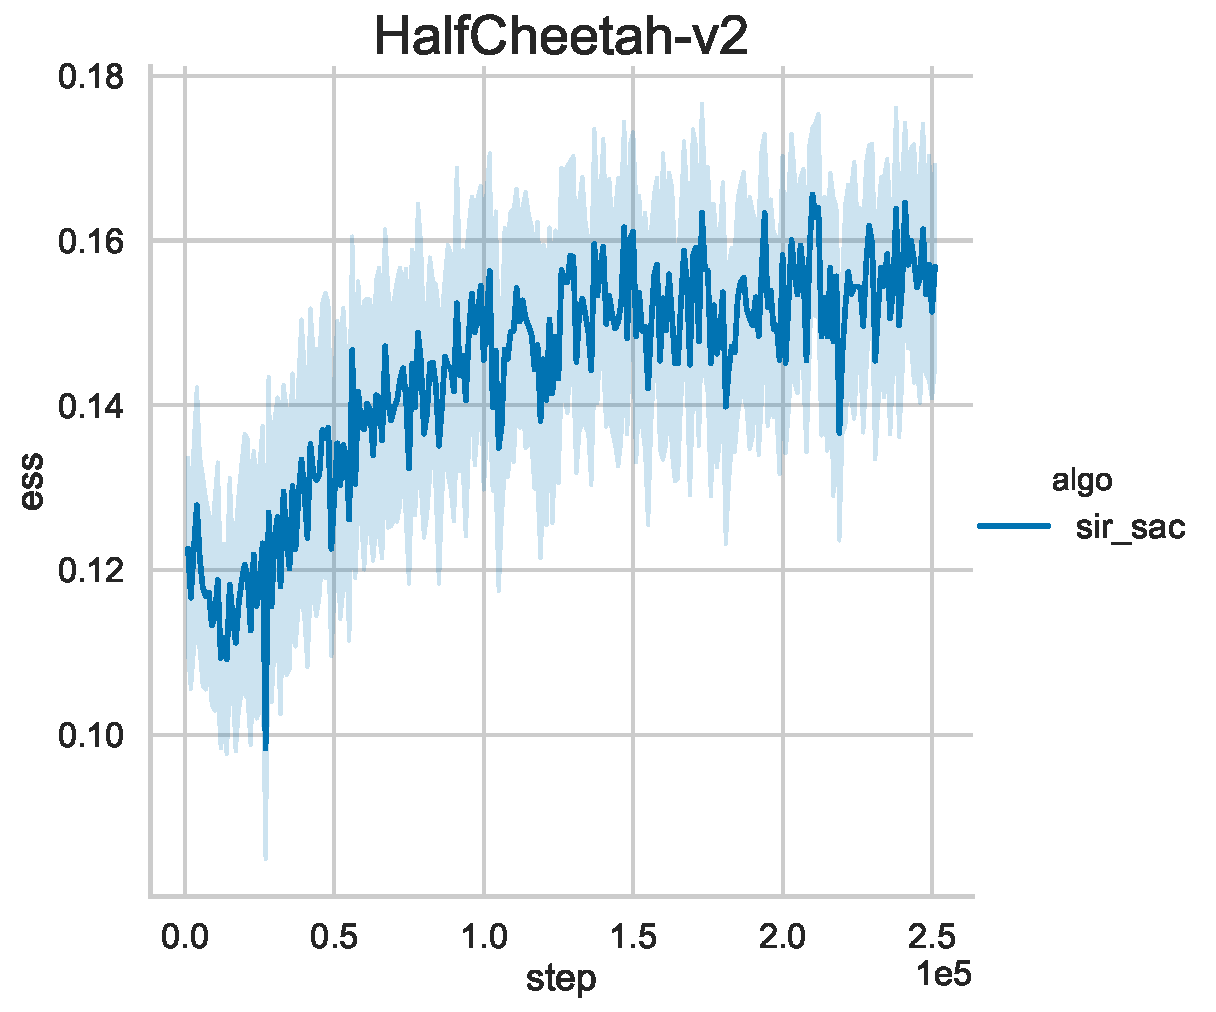
\includegraphics[width=0.5\linewidth]{articles/smcp/figures/HalfCheetah-v2_ess1543280008.pdf}
\caption{Effective sample size for HalfCheetah. The shaded area represents the standard deviation over 20 seeds.}
\label{fig:ess}
\end{figure}

% The normalized effective sample size (ESS) is reported in Figure \ref{fig:ess}. 

The values reported on Figure \ref{fig:ess} are the harmonic mean of the ratio of the effective sample size by the actual number of particles.

More precisely the values are
$$y_t =  \big(\prod_{i=1}^{h} \text{ESS}_i(t) / N \big)^{1/h}$$
where $i$ is the depth of the planning, $N$ is the number of particles and 
$$\text{ESS}_i(t) = \frac{(\sum_{n=1}^N w_{t+i}^{(n)})^2}{\sum_{n=1}^N (w_{t+i}^{(n)})^2}$$ 

We can see that as the proposal distribution improves the ESS also increases. The ESS on HalfCheetah is representative of the one obtained on the other environments. 
While these values are not high, we are still around $15 \%$ thus we do not suffer heavily from weight degeneracy. 


\subsubsection{Model loss}
\label{app:model_loss}
We also report the negative log likelihood loss of the environment's model during the training on Figure~\ref{fig:neg_log_lik}.


\begin{figure}[!h]
\centering
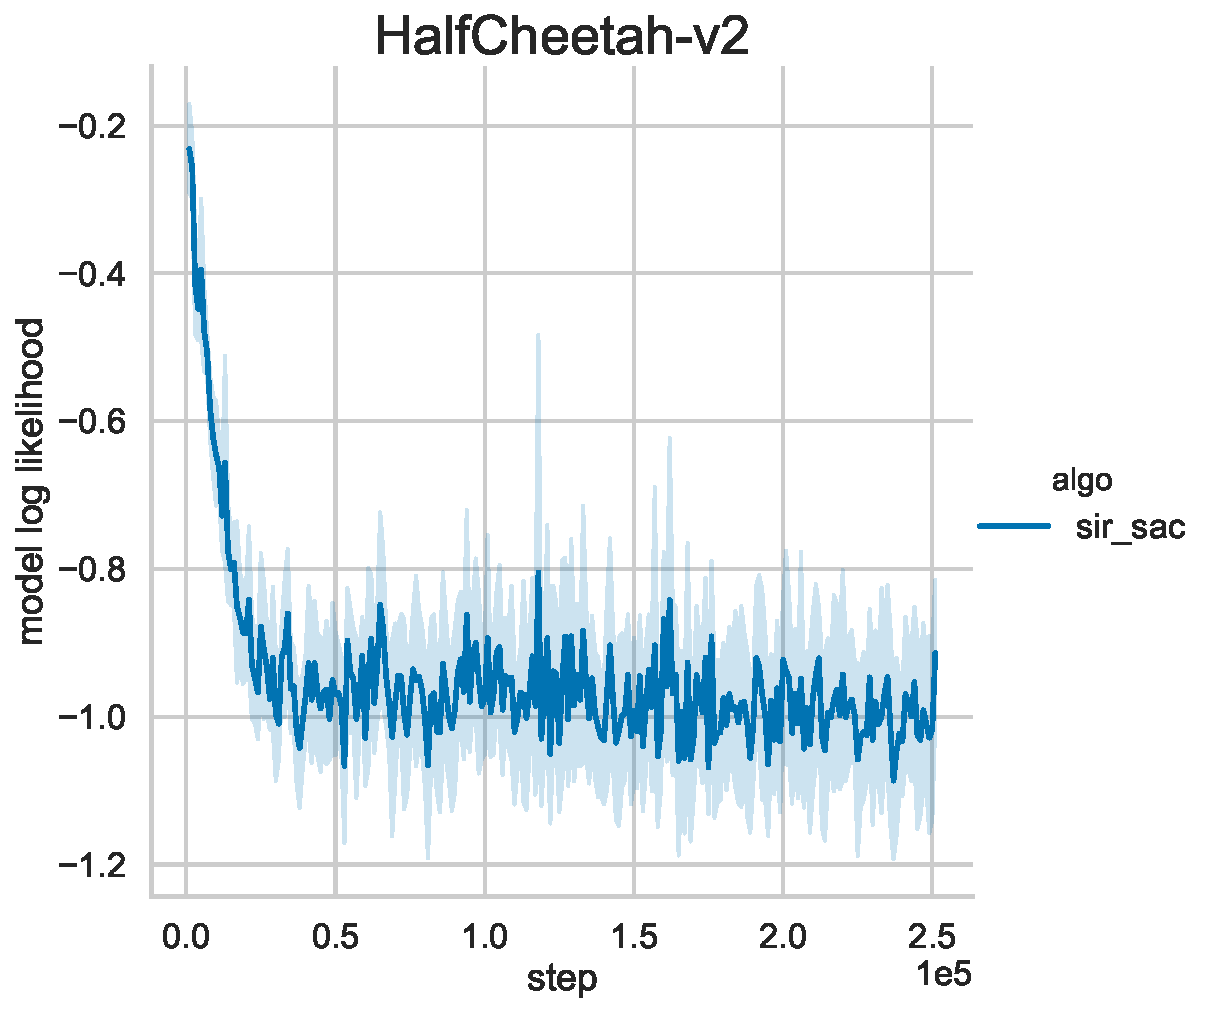
\includegraphics[width=0.5\linewidth]{articles/smcp/figures/HalfCheetah-v2_loglik1543284334.pdf}
\caption{Negative log likelihood for the model on HalfCheetah. The shaded area represents the standard deviation over 20 seeds.}
\label{fig:neg_log_lik}
\end{figure}
